\documentclass[12pt,]{article}
\usepackage{lmodern}
\usepackage{amssymb,amsmath}
\usepackage{ifxetex,ifluatex}
\usepackage{fixltx2e} % provides \textsubscript
\ifnum 0\ifxetex 1\fi\ifluatex 1\fi=0 % if pdftex
  \usepackage[T1]{fontenc}
  \usepackage[utf8]{inputenc}
\else % if luatex or xelatex
  \ifxetex
    \usepackage{mathspec}
  \else
    \usepackage{fontspec}
  \fi
  \defaultfontfeatures{Ligatures=TeX,Scale=MatchLowercase}
    \setmainfont[]{Times New Roman}
\fi
% use upquote if available, for straight quotes in verbatim environments
\IfFileExists{upquote.sty}{\usepackage{upquote}}{}
% use microtype if available
\IfFileExists{microtype.sty}{%
\usepackage{microtype}
\UseMicrotypeSet[protrusion]{basicmath} % disable protrusion for tt fonts
}{}
\usepackage[margin=2.54cm]{geometry}
\usepackage{hyperref}
\hypersetup{unicode=true,
            pdftitle={Trends in Alternative Daily Cover in California},
            pdfauthor={Sarah Ko},
            pdfborder={0 0 0},
            breaklinks=true}
\urlstyle{same}  % don't use monospace font for urls
\usepackage{color}
\usepackage{fancyvrb}
\newcommand{\VerbBar}{|}
\newcommand{\VERB}{\Verb[commandchars=\\\{\}]}
\DefineVerbatimEnvironment{Highlighting}{Verbatim}{commandchars=\\\{\}}
% Add ',fontsize=\small' for more characters per line
\usepackage{framed}
\definecolor{shadecolor}{RGB}{248,248,248}
\newenvironment{Shaded}{\begin{snugshade}}{\end{snugshade}}
\newcommand{\KeywordTok}[1]{\textcolor[rgb]{0.13,0.29,0.53}{\textbf{#1}}}
\newcommand{\DataTypeTok}[1]{\textcolor[rgb]{0.13,0.29,0.53}{#1}}
\newcommand{\DecValTok}[1]{\textcolor[rgb]{0.00,0.00,0.81}{#1}}
\newcommand{\BaseNTok}[1]{\textcolor[rgb]{0.00,0.00,0.81}{#1}}
\newcommand{\FloatTok}[1]{\textcolor[rgb]{0.00,0.00,0.81}{#1}}
\newcommand{\ConstantTok}[1]{\textcolor[rgb]{0.00,0.00,0.00}{#1}}
\newcommand{\CharTok}[1]{\textcolor[rgb]{0.31,0.60,0.02}{#1}}
\newcommand{\SpecialCharTok}[1]{\textcolor[rgb]{0.00,0.00,0.00}{#1}}
\newcommand{\StringTok}[1]{\textcolor[rgb]{0.31,0.60,0.02}{#1}}
\newcommand{\VerbatimStringTok}[1]{\textcolor[rgb]{0.31,0.60,0.02}{#1}}
\newcommand{\SpecialStringTok}[1]{\textcolor[rgb]{0.31,0.60,0.02}{#1}}
\newcommand{\ImportTok}[1]{#1}
\newcommand{\CommentTok}[1]{\textcolor[rgb]{0.56,0.35,0.01}{\textit{#1}}}
\newcommand{\DocumentationTok}[1]{\textcolor[rgb]{0.56,0.35,0.01}{\textbf{\textit{#1}}}}
\newcommand{\AnnotationTok}[1]{\textcolor[rgb]{0.56,0.35,0.01}{\textbf{\textit{#1}}}}
\newcommand{\CommentVarTok}[1]{\textcolor[rgb]{0.56,0.35,0.01}{\textbf{\textit{#1}}}}
\newcommand{\OtherTok}[1]{\textcolor[rgb]{0.56,0.35,0.01}{#1}}
\newcommand{\FunctionTok}[1]{\textcolor[rgb]{0.00,0.00,0.00}{#1}}
\newcommand{\VariableTok}[1]{\textcolor[rgb]{0.00,0.00,0.00}{#1}}
\newcommand{\ControlFlowTok}[1]{\textcolor[rgb]{0.13,0.29,0.53}{\textbf{#1}}}
\newcommand{\OperatorTok}[1]{\textcolor[rgb]{0.81,0.36,0.00}{\textbf{#1}}}
\newcommand{\BuiltInTok}[1]{#1}
\newcommand{\ExtensionTok}[1]{#1}
\newcommand{\PreprocessorTok}[1]{\textcolor[rgb]{0.56,0.35,0.01}{\textit{#1}}}
\newcommand{\AttributeTok}[1]{\textcolor[rgb]{0.77,0.63,0.00}{#1}}
\newcommand{\RegionMarkerTok}[1]{#1}
\newcommand{\InformationTok}[1]{\textcolor[rgb]{0.56,0.35,0.01}{\textbf{\textit{#1}}}}
\newcommand{\WarningTok}[1]{\textcolor[rgb]{0.56,0.35,0.01}{\textbf{\textit{#1}}}}
\newcommand{\AlertTok}[1]{\textcolor[rgb]{0.94,0.16,0.16}{#1}}
\newcommand{\ErrorTok}[1]{\textcolor[rgb]{0.64,0.00,0.00}{\textbf{#1}}}
\newcommand{\NormalTok}[1]{#1}
\usepackage{graphicx,grffile}
\makeatletter
\def\maxwidth{\ifdim\Gin@nat@width>\linewidth\linewidth\else\Gin@nat@width\fi}
\def\maxheight{\ifdim\Gin@nat@height>\textheight\textheight\else\Gin@nat@height\fi}
\makeatother
% Scale images if necessary, so that they will not overflow the page
% margins by default, and it is still possible to overwrite the defaults
% using explicit options in \includegraphics[width, height, ...]{}
\setkeys{Gin}{width=\maxwidth,height=\maxheight,keepaspectratio}
\IfFileExists{parskip.sty}{%
\usepackage{parskip}
}{% else
\setlength{\parindent}{0pt}
\setlength{\parskip}{6pt plus 2pt minus 1pt}
}
\setlength{\emergencystretch}{3em}  % prevent overfull lines
\providecommand{\tightlist}{%
  \setlength{\itemsep}{0pt}\setlength{\parskip}{0pt}}
\setcounter{secnumdepth}{5}
% Redefines (sub)paragraphs to behave more like sections
\ifx\paragraph\undefined\else
\let\oldparagraph\paragraph
\renewcommand{\paragraph}[1]{\oldparagraph{#1}\mbox{}}
\fi
\ifx\subparagraph\undefined\else
\let\oldsubparagraph\subparagraph
\renewcommand{\subparagraph}[1]{\oldsubparagraph{#1}\mbox{}}
\fi

%%% Use protect on footnotes to avoid problems with footnotes in titles
\let\rmarkdownfootnote\footnote%
\def\footnote{\protect\rmarkdownfootnote}

%%% Change title format to be more compact
\usepackage{titling}

% Create subtitle command for use in maketitle
\providecommand{\subtitle}[1]{
  \posttitle{
    \begin{center}\large#1\end{center}
    }
}

\setlength{\droptitle}{-2em}

  \title{Trends in Alternative Daily Cover in California}
    \pretitle{\vspace{\droptitle}\centering\huge}
  \posttitle{\par}
  \subtitle{\url{https://github.com/sarahko7/ADC_Analysis}}
  \author{Sarah Ko}
    \preauthor{\centering\large\emph}
  \postauthor{\par}
    \date{}
    \predate{}\postdate{}
  
\usepackage{booktabs}
\usepackage{longtable}
\usepackage{array}
\usepackage{multirow}
\usepackage{wrapfig}
\usepackage{float}
\usepackage{colortbl}
\usepackage{pdflscape}
\usepackage{tabu}
\usepackage{threeparttable}
\usepackage{threeparttablex}
\usepackage[normalem]{ulem}
\usepackage{makecell}
\usepackage{xcolor}

\begin{document}
\maketitle
\begin{abstract}
Experimental overview. This section should be no longer than 250 words.
\end{abstract}

\newpage

\tableofcontents 

\newpage

\listoftables 

\newpage

\listoffigures 

\newpage

\textless{}Note: set up autoreferencing for figures and tables in your
document\textgreater{}

\section{Research Question and
Rationale}\label{research-question-and-rationale}

\newpage

\section{Dataset Information}\label{anchor}

\begin{table}[H]
\centering
\begin{tabular}{l|l}
\hline
\textbf{Column Name} & \textbf{Data Description}\\
\hline
Report Year & Year that the ADC was used\\
\hline
Report Quarter & Quarter that the ADC was used\\
\hline
Ash & Ash and cement kiln dust materials\\
\hline
Auto Shredder Waste & Treated auto shredder waste\\
\hline
Construction and Demolition Waste & Processed construction and demolition wastes and materials\\
\hline
Compost & Compost materials\\
\hline
Contaminated Sediment & Contaminated sediment, dredge spoils, foundry sands\\
\hline
Green Material & Processed green material\\
\hline
Mixed & Mixtures of the other categories\\
\hline
Other & Before 1998, most ADC was classified in this category\\
\hline
Tires & Shredded tires\\
\hline
Sludge & Sludge and sludge-derived materials\\
\hline
Total & Sum of the columns Ash:Sludge\\
\hline
\end{tabular}
\end{table}

SKOTESTThis is the caption for the table Table 1: Summary of Data
Structure

SKOTESTreference the table in text: Table 1

\newpage

\section{Exploratory Data Analysis and
Wrangling}\label{exploratory-data-analysis-and-wrangling}

\subsection{Import \& Explore}\label{import-explore}

\begin{Shaded}
\begin{Highlighting}[]
\CommentTok{# import dataset}
\NormalTok{ADC_raw <-}\StringTok{ }\KeywordTok{read.csv}\NormalTok{(}\StringTok{"../Raw_Data/CalRecycle_ADC_raw.csv"}\NormalTok{)}

\CommentTok{# explore dataset}
\KeywordTok{view}\NormalTok{(ADC_raw)}
\KeywordTok{class}\NormalTok{(ADC_raw)}
\end{Highlighting}
\end{Shaded}

\begin{verbatim}
## [1] "data.frame"
\end{verbatim}

\begin{Shaded}
\begin{Highlighting}[]
\KeywordTok{colnames}\NormalTok{(ADC_raw)}
\end{Highlighting}
\end{Shaded}

\begin{verbatim}
##  [1] "Report.Year"                      
##  [2] "Report.Quarter"                   
##  [3] "Ash"                              
##  [4] "Auto.Shredder.Waste"              
##  [5] "Construction.and.Demolition.Waste"
##  [6] "Compost"                          
##  [7] "Contaminated.Sediment"            
##  [8] "Green.Material"                   
##  [9] "Mixed"                            
## [10] "Other"                            
## [11] "Tires"                            
## [12] "Sludge"                           
## [13] "Total"
\end{verbatim}

\begin{Shaded}
\begin{Highlighting}[]
\KeywordTok{dim}\NormalTok{(ADC_raw)}
\end{Highlighting}
\end{Shaded}

\begin{verbatim}
## [1] 92 13
\end{verbatim}

\begin{Shaded}
\begin{Highlighting}[]
\CommentTok{# per the CalRecycle website, segregation into ADC types started in 1998}
\CommentTok{# therefore, for the analysis, remove data from before 1998}
\KeywordTok{class}\NormalTok{(ADC_raw}\OperatorTok{$}\NormalTok{Report.Year)}
\end{Highlighting}
\end{Shaded}

\begin{verbatim}
## [1] "integer"
\end{verbatim}

\begin{Shaded}
\begin{Highlighting}[]
\NormalTok{ADC_data <-}\StringTok{ }\KeywordTok{filter}\NormalTok{(ADC_raw, Report.Year }\OperatorTok{>=}\StringTok{ }\DecValTok{1998}\NormalTok{)}
\KeywordTok{dim}\NormalTok{(ADC_data)}
\end{Highlighting}
\end{Shaded}

\begin{verbatim}
## [1] 80 13
\end{verbatim}

\begin{Shaded}
\begin{Highlighting}[]
\CommentTok{# explore new dataset}
\KeywordTok{head}\NormalTok{(ADC_data)}
\end{Highlighting}
\end{Shaded}

\begin{verbatim}
##   Report.Year Report.Quarter      Ash Auto.Shredder.Waste
## 1        2017              1 32511.83            153270.6
## 2        2017              2 37294.78            159759.7
## 3        2017              3 33349.25            153342.6
## 4        2017              4 22248.85            123203.5
## 5        2016              1 31423.40            123193.3
## 6        2016              2 45504.45            126040.9
##   Construction.and.Demolition.Waste  Compost Contaminated.Sediment
## 1                          173548.6  6128.89               3396.36
## 2                          199486.8  2746.22               7585.58
## 3                          164028.4  1796.97               4280.92
## 4                          198901.7 15993.13               2979.12
## 5                          160446.5 15681.63              20203.18
## 6                          144982.9 42215.62              18089.73
##   Green.Material    Mixed    Other   Tires    Sludge    Total
## 1       380686.2     0.00 71983.68 3771.40  68063.34 893360.9
## 2       401034.3  1516.12 71066.46 5066.35  65585.25 951141.6
## 3       362474.4 10891.73 78980.55 5323.75  79967.05 894435.6
## 4       347204.0  7964.83 56849.63 4575.75 141423.92 921344.5
## 5       334512.7 12756.90 82081.97 3402.03  83424.85 867126.5
## 6       310959.5 17946.71 75803.52 3616.26  72882.61 858042.2
\end{verbatim}

\begin{Shaded}
\begin{Highlighting}[]
\KeywordTok{tail}\NormalTok{(ADC_data)}
\end{Highlighting}
\end{Shaded}

\begin{verbatim}
##    Report.Year Report.Quarter     Ash Auto.Shredder.Waste
## 75        1999              3 1578.70            69300.25
## 76        1999              4 2718.22            63910.19
## 77        1998              1 2631.85            39181.17
## 78        1998              2  878.63            49391.25
## 79        1998              3 2457.00            35573.00
## 80        1998              4 2418.00            38495.89
##    Construction.and.Demolition.Waste Compost Contaminated.Sediment
## 75                          48321.13       0                  0.00
## 76                          62057.02     381                 16.50
## 77                           2693.48       0                  0.00
## 78                           6666.70       0                  2.74
## 79                          28278.30       0                 92.17
## 80                          29591.80       0                  0.00
##    Green.Material   Mixed   Other    Tires   Sludge    Total
## 75       349276.6    0.00 4695.69  1265.82 66864.38 541302.6
## 76       360153.2    0.00 6316.72  3307.48 69058.27 567918.6
## 77       191066.3 3907.20 1008.27 14802.71 43391.12 298682.1
## 78       279191.3 3602.22 3305.93 15394.54 92416.47 450849.8
## 79       299986.8    0.00 2706.53  2943.31 99312.34 471349.4
## 80       313452.3 4130.00 3767.93   733.71 57511.25 450100.9
\end{verbatim}

\begin{Shaded}
\begin{Highlighting}[]
\CommentTok{# tidy the data by gathering the type columns}
\NormalTok{ADC_gathered <-}\StringTok{ }\KeywordTok{gather}\NormalTok{(ADC_data, }\StringTok{"Type"}\NormalTok{, }\StringTok{"Quantity"}\NormalTok{, Ash}\OperatorTok{:}\NormalTok{Sludge) }\OperatorTok
\StringTok{  }\KeywordTok{select}\NormalTok{(}\OperatorTok{-}\NormalTok{Total) }\CommentTok{# remove Total column}

\CommentTok{# save the tidy dataset}
\KeywordTok{write.csv}\NormalTok{(ADC_data, }\DataTypeTok{row.names =} \OtherTok{FALSE}\NormalTok{, }\DataTypeTok{file =} \StringTok{"../Processed_Data/CalRecycle_ADC_tidy_processed.csv"}\NormalTok{)}

\CommentTok{# generate summary data}
\NormalTok{ADC_summary_by_type <-}\StringTok{ }\NormalTok{ADC_gathered }\OperatorTok
\StringTok{  }\KeywordTok{group_by}\NormalTok{(Type) }\OperatorTok\StringTok{ }\CommentTok{# group the data by lakename}
\StringTok{  }\KeywordTok{filter}\NormalTok{(}\OperatorTok{!}\KeywordTok{is.na}\NormalTok{(Quantity)) }\OperatorTok\StringTok{ }\CommentTok{#remove the records when there are nas Quantity}
\StringTok{  }\KeywordTok{summarise}\NormalTok{(}\DataTypeTok{MeanQuarterlyQuantity =} \KeywordTok{mean}\NormalTok{(Quantity), }
            \DataTypeTok{MinQuarterlyQuantity =} \KeywordTok{min}\NormalTok{(Quantity), }
            \DataTypeTok{MaxQuarterlyQuantity =} \KeywordTok{max}\NormalTok{(Quantity), }
            \DataTypeTok{sdQuarterlyQuantity =} \KeywordTok{sd}\NormalTok{(Quantity), }
            \DataTypeTok{medianQuarterlyQuantity =} \KeywordTok{median}\NormalTok{(Quantity))}

\NormalTok{ADC_summary_by_year <-}\StringTok{ }\NormalTok{ADC_gathered }\OperatorTok
\StringTok{  }\KeywordTok{group_by}\NormalTok{(Report.Year) }\OperatorTok\StringTok{ }\CommentTok{# group the data by year}
\StringTok{  }\KeywordTok{filter}\NormalTok{(}\OperatorTok{!}\KeywordTok{is.na}\NormalTok{(Quantity)) }\OperatorTok\StringTok{ }\CommentTok{#remove the records when there are nas Quantity}
\StringTok{  }\KeywordTok{summarise}\NormalTok{(}\DataTypeTok{MeanQuarterlyQuantity =} \KeywordTok{mean}\NormalTok{(Quantity), }
            \DataTypeTok{MinQuarterlyQuantity =} \KeywordTok{min}\NormalTok{(Quantity), }
            \DataTypeTok{MaxQuarterlyQuantity =} \KeywordTok{max}\NormalTok{(Quantity), }
            \DataTypeTok{sdQuarterlyQuantity =} \KeywordTok{sd}\NormalTok{(Quantity), }
            \DataTypeTok{medianQuarterlyQuantity =} \KeywordTok{median}\NormalTok{(Quantity))}
\end{Highlighting}
\end{Shaded}

\subsection{Create Graphs}\label{create-graphs}

\begin{Shaded}
\begin{Highlighting}[]
\CommentTok{# Graph 1: for 2017 data, display total by type}
\NormalTok{total_bytype_}\DecValTok{2017}\NormalTok{ <-}\StringTok{ }\NormalTok{ADC_gathered }\OperatorTok
\StringTok{  }\KeywordTok{filter}\NormalTok{(Report.Year }\OperatorTok{==}\StringTok{ }\DecValTok{2017}\NormalTok{) }\OperatorTok
\StringTok{  }\KeywordTok{group_by}\NormalTok{(Type) }\OperatorTok
\StringTok{  }\KeywordTok{summarize}\NormalTok{(}\DataTypeTok{Quantity =} \KeywordTok{sum}\NormalTok{(Quantity))}

\CommentTok{# save 2017 dataset}
\KeywordTok{write.csv}\NormalTok{(total_bytype_}\DecValTok{2017}\NormalTok{, }\DataTypeTok{row.names =} \OtherTok{FALSE}\NormalTok{, }\DataTypeTok{file =} \StringTok{"../Processed_Data/CalRecycle_ADC_2017only_processed.csv"}\NormalTok{)}

\CommentTok{# convert column Type into factor}
\KeywordTok{class}\NormalTok{(total_bytype_}\DecValTok{2017}\OperatorTok{$}\NormalTok{Type)}
\end{Highlighting}
\end{Shaded}

\begin{verbatim}
## [1] "character"
\end{verbatim}

\begin{Shaded}
\begin{Highlighting}[]
\NormalTok{total_bytype_}\DecValTok{2017}\OperatorTok{$}\NormalTok{Type <-}\StringTok{ }\KeywordTok{as.factor}\NormalTok{(total_bytype_}\DecValTok{2017}\OperatorTok{$}\NormalTok{Type)}

\CommentTok{# plot as a bar chart}
\NormalTok{total_bytype_2017_plot <-}\StringTok{ }
\StringTok{    }\KeywordTok{ggplot}\NormalTok{(}\DataTypeTok{data=}\NormalTok{total_bytype_}\DecValTok{2017}\NormalTok{, }\KeywordTok{aes}\NormalTok{(}\DataTypeTok{x=}\NormalTok{Type, }\DataTypeTok{y=}\NormalTok{Quantity)) }\OperatorTok{+}
\StringTok{    }\KeywordTok{geom_bar}\NormalTok{(}\DataTypeTok{stat=}\StringTok{"identity"}\NormalTok{) }\OperatorTok{+}\StringTok{ }
\StringTok{    }\KeywordTok{xlab}\NormalTok{(}\StringTok{''}\NormalTok{) }\OperatorTok{+}\StringTok{ }
\StringTok{    }\KeywordTok{ylab}\NormalTok{(}\StringTok{"Quantity (U.S. Tons)"}\NormalTok{) }\OperatorTok{+}
\StringTok{    }\KeywordTok{ggtitle}\NormalTok{(}\StringTok{"2017 Quantities of ADC by Type"}\NormalTok{) }\OperatorTok{+}
\StringTok{    }\KeywordTok{theme}\NormalTok{(}\DataTypeTok{axis.text.x =} \KeywordTok{element_text}\NormalTok{(}\DataTypeTok{angle =} \DecValTok{45}\NormalTok{, }\DataTypeTok{hjust =} \DecValTok{1}\NormalTok{)) }\OperatorTok{+}\StringTok{ }
\StringTok{    }\KeywordTok{scale_x_discrete}\NormalTok{(}\DataTypeTok{labels =} \KeywordTok{c}\NormalTok{(}\StringTok{'Ash'}\NormalTok{,}\StringTok{'Auto Shredder Waste'}\NormalTok{,}\StringTok{'Compost'}\NormalTok{, }\StringTok{'Construction & Demolition Waste'}\NormalTok{, }\StringTok{'Contaminated Sediment'}\NormalTok{, }\StringTok{'Green Material'}\NormalTok{, }\StringTok{'Mixed'}\NormalTok{, }\StringTok{'Other'}\NormalTok{, }\StringTok{'Sludge'}\NormalTok{, }\StringTok{'Tires'}\NormalTok{))}
\KeywordTok{print}\NormalTok{(total_bytype_2017_plot)}
\end{Highlighting}
\end{Shaded}

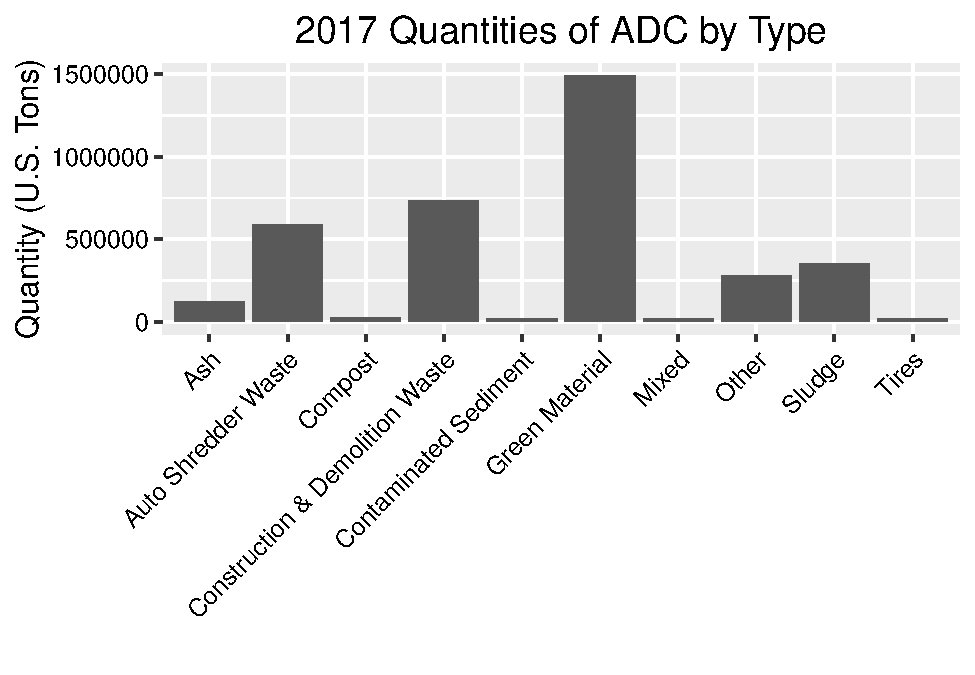
\includegraphics{SKo_Project_Template_files/figure-latex/explore_graphs-1.pdf}

\begin{Shaded}
\begin{Highlighting}[]
\CommentTok{# save figure}
\KeywordTok{ggsave}\NormalTok{(}\StringTok{"2017ADCbytype_alltypes.jpg"}\NormalTok{, total_bytype_2017_plot, }\DataTypeTok{path =} \StringTok{"../Output"}\NormalTok{, }\DataTypeTok{height =} \DecValTok{4}\NormalTok{, }\DataTypeTok{width =} \DecValTok{6}\NormalTok{, }\DataTypeTok{units =} \StringTok{"in"}\NormalTok{, }\DataTypeTok{dpi =} \DecValTok{300}\NormalTok{)}

\CommentTok{# Graph 2: faceted by Type, display spread of quarterly values by year}
\NormalTok{quarterlyvalues_byyear_plot <-}\StringTok{ }\KeywordTok{ggplot}\NormalTok{(ADC_gathered) }\OperatorTok{+}
\StringTok{  }\KeywordTok{geom_boxplot}\NormalTok{(}\KeywordTok{aes}\NormalTok{(}\DataTypeTok{x =}\NormalTok{ Report.Year, }\DataTypeTok{y =}\NormalTok{ Quantity, }\DataTypeTok{group =}\NormalTok{ Report.Year)) }\OperatorTok{+}\StringTok{ }
\StringTok{  }\KeywordTok{facet_wrap}\NormalTok{(}\KeywordTok{vars}\NormalTok{(Type), }\DataTypeTok{nrow =} \DecValTok{5}\NormalTok{) }\OperatorTok{+}\StringTok{ }
\StringTok{  }\KeywordTok{xlab}\NormalTok{(}\StringTok{""}\NormalTok{) }\OperatorTok{+}
\StringTok{  }\KeywordTok{ylab}\NormalTok{(}\StringTok{"Quarterly Quantity (U.S. Tons)"}\NormalTok{) }\OperatorTok{+}
\StringTok{  }\KeywordTok{ggtitle}\NormalTok{(}\StringTok{"Quarterly Quantities of ADC, Grouped by Year"}\NormalTok{)}
\KeywordTok{print}\NormalTok{(quarterlyvalues_byyear_plot)}
\end{Highlighting}
\end{Shaded}

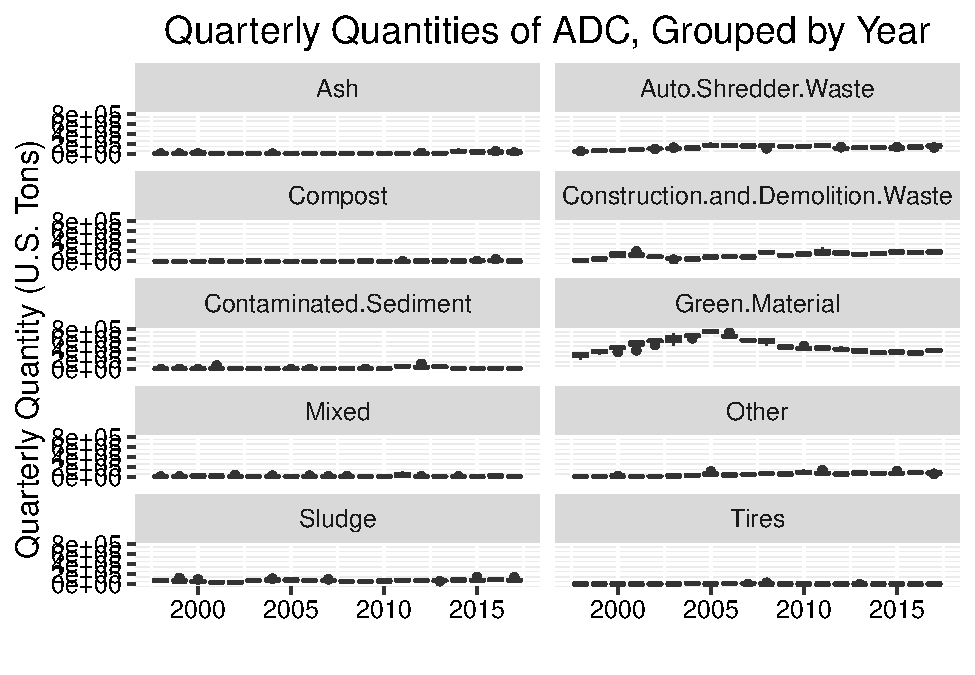
\includegraphics{SKo_Project_Template_files/figure-latex/explore_graphs-2.pdf}

\begin{Shaded}
\begin{Highlighting}[]
\CommentTok{# save figure}
\KeywordTok{ggsave}\NormalTok{(}\StringTok{"ADCyeardistribution_alltypes.jpg"}\NormalTok{, quarterlyvalues_byyear_plot, }\DataTypeTok{path =} \StringTok{"../Output"}\NormalTok{, }\DataTypeTok{height =} \DecValTok{8}\NormalTok{, }\DataTypeTok{width =} \DecValTok{8}\NormalTok{, }\DataTypeTok{units =} \StringTok{"in"}\NormalTok{, }\DataTypeTok{dpi =} \DecValTok{300}\NormalTok{)}

\CommentTok{# Graph 3: display data by quarter, all Types on same plot}
\NormalTok{quarterlyvalues_alltypes_plot <-}\StringTok{ }
\StringTok{  }\KeywordTok{ggplot}\NormalTok{(ADC_gathered) }\OperatorTok{+}\StringTok{ }
\StringTok{  }\KeywordTok{geom_jitter}\NormalTok{(}\KeywordTok{aes}\NormalTok{(}\DataTypeTok{x =}\NormalTok{ Report.Quarter, }\DataTypeTok{y =}\NormalTok{ Quantity, }\DataTypeTok{shape =} \KeywordTok{as.factor}\NormalTok{(Type), }\DataTypeTok{color =} \KeywordTok{as.factor}\NormalTok{(Report.Year)), }\DataTypeTok{width =} \FloatTok{0.3}\NormalTok{, }\DataTypeTok{height =} \DecValTok{0}\NormalTok{) }\OperatorTok{+}\StringTok{ }
\StringTok{  }\KeywordTok{labs}\NormalTok{(}\DataTypeTok{shape=}\StringTok{"Type"}\NormalTok{, }\DataTypeTok{colour=}\StringTok{"Year"}\NormalTok{) }\OperatorTok{+}\StringTok{ }
\StringTok{  }\KeywordTok{xlab}\NormalTok{(}\StringTok{"Quarter"}\NormalTok{) }\OperatorTok{+}\StringTok{ }
\StringTok{  }\KeywordTok{ylab}\NormalTok{(}\StringTok{"Quantity (U.S. Tons)"}\NormalTok{) }\OperatorTok{+}\StringTok{ }
\StringTok{  }\KeywordTok{ggtitle}\NormalTok{(}\StringTok{"Quantities Within Quarters"}\NormalTok{) }\OperatorTok{+}\StringTok{ }
\StringTok{  }\KeywordTok{scale_shape_manual}\NormalTok{(}\DataTypeTok{values=}\KeywordTok{c}\NormalTok{(}\DecValTok{1}\NormalTok{, }\DecValTok{2}\NormalTok{, }\DecValTok{3}\NormalTok{, }\DecValTok{4}\NormalTok{, }\DecValTok{5}\NormalTok{, }\DecValTok{6}\NormalTok{, }\DecValTok{7}\NormalTok{, }\DecValTok{8}\NormalTok{, }\DecValTok{9}\NormalTok{, }\DecValTok{10}\NormalTok{), }\DataTypeTok{labels =} \KeywordTok{c}\NormalTok{(}\StringTok{"Ash"}\NormalTok{, }\StringTok{"Auto Shredder Waste"}\NormalTok{, }\StringTok{"Compost"}\NormalTok{, }\StringTok{"Construction & Demolition"}\NormalTok{, }\StringTok{"Contaminated Sediment"}\NormalTok{, }\StringTok{"Green Material"}\NormalTok{, }\StringTok{"Mixed"}\NormalTok{, }\StringTok{"Other"}\NormalTok{, }\StringTok{"Sludge"}\NormalTok{, }\StringTok{"Tires"}\NormalTok{)) }\OperatorTok{+}\StringTok{ }
\StringTok{  }\KeywordTok{theme}\NormalTok{(}\DataTypeTok{legend.position=}\StringTok{"right"}\NormalTok{, }\DataTypeTok{legend.box =} \StringTok{"vertical"}\NormalTok{, }\DataTypeTok{legend.direction =} \StringTok{"vertical"}\NormalTok{) }\OperatorTok{+}\StringTok{ }
\StringTok{  }\KeywordTok{guides}\NormalTok{(}\DataTypeTok{shape =} \KeywordTok{guide_legend}\NormalTok{(}\DataTypeTok{order =} \DecValTok{1}\NormalTok{), }\DataTypeTok{color =} \KeywordTok{guide_legend}\NormalTok{(}\DataTypeTok{order =} \DecValTok{2}\NormalTok{))}
\KeywordTok{print}\NormalTok{(quarterlyvalues_alltypes_plot)}
\end{Highlighting}
\end{Shaded}

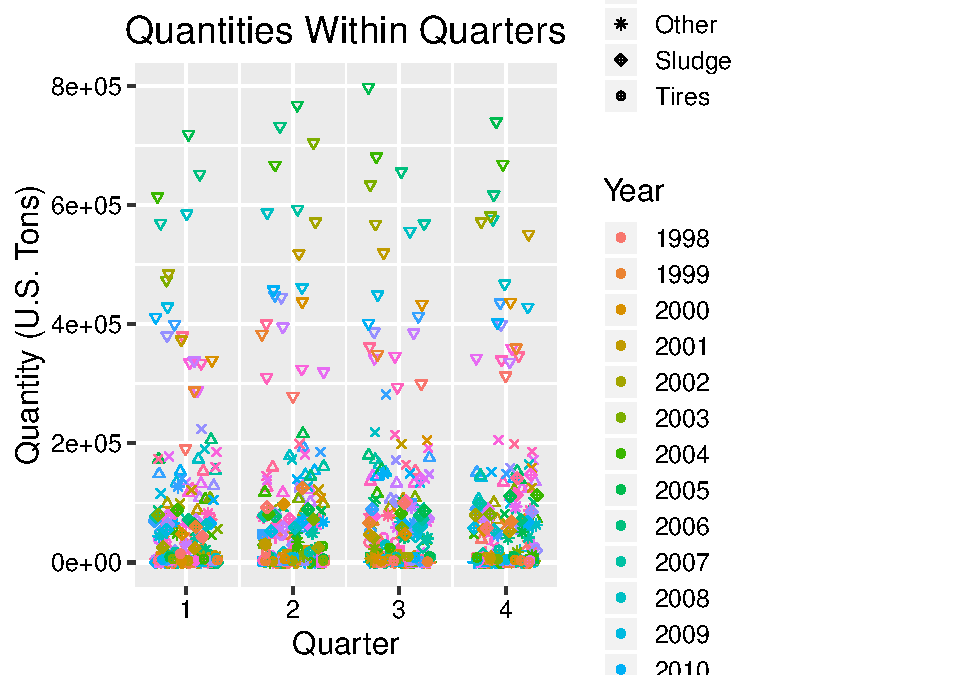
\includegraphics{SKo_Project_Template_files/figure-latex/explore_graphs-3.pdf}

\begin{Shaded}
\begin{Highlighting}[]
\CommentTok{# save figure}
\KeywordTok{ggsave}\NormalTok{(}\StringTok{"QuarterlyADC_alltypes.jpg"}\NormalTok{, quarterlyvalues_alltypes_plot, }\DataTypeTok{path =} \StringTok{"../Output"}\NormalTok{, }\DataTypeTok{height =} \DecValTok{9}\NormalTok{, }\DataTypeTok{width =} \DecValTok{9}\NormalTok{, }\DataTypeTok{units =} \StringTok{"in"}\NormalTok{, }\DataTypeTok{dpi =} \DecValTok{300}\NormalTok{)}
\end{Highlighting}
\end{Shaded}

\newpage

\section{Analysis}\label{analysis}

\subsection{Test 1: Statistical Modeling \& Data
Visualization}\label{test-1-statistical-modeling-data-visualization}

Is there a significant difference in total ADC between report quarters?
(i.e.~1, 2, 3, 4)

\begin{Shaded}
\begin{Highlighting}[]
\CommentTok{# create dataset with only total values, from 1995-2017}
\NormalTok{ADC_total_only <-}\StringTok{ }\NormalTok{ADC_raw }\OperatorTok
\StringTok{  }\KeywordTok{select}\NormalTok{(Report.Year, Report.Quarter, Total) }\CommentTok{# keep all columns except ADC Types}

\CommentTok{# convert column Report.Quarter into factor}
\KeywordTok{class}\NormalTok{(ADC_total_only}\OperatorTok{$}\NormalTok{Report.Quarter)}
\end{Highlighting}
\end{Shaded}

\begin{verbatim}
## [1] "integer"
\end{verbatim}

\begin{Shaded}
\begin{Highlighting}[]
\NormalTok{ADC_total_only}\OperatorTok{$}\NormalTok{Report.Quarter <-}\StringTok{ }\KeywordTok{as.factor}\NormalTok{(ADC_total_only}\OperatorTok{$}\NormalTok{Report.Quarter) }

\CommentTok{# save the dataset}
\KeywordTok{write.csv}\NormalTok{(ADC_total_only, }\DataTypeTok{row.names =} \OtherTok{FALSE}\NormalTok{, }\DataTypeTok{file =} \StringTok{"../Processed_Data/CalRecycle_ADC_totalsonly_processed.csv"}\NormalTok{)}

\CommentTok{# perform one-way ANOVA}
\CommentTok{# assumption #0: observations are independent (cannot be tested, but assumed to be independent)}

\CommentTok{# test assumption #1: normality}
\CommentTok{# null hypothesis is that the dataset is normally distributed}
\KeywordTok{shapiro.test}\NormalTok{(ADC_total_only}\OperatorTok{$}\NormalTok{Total[ADC_total_only}\OperatorTok{$}\NormalTok{Report.Quarter }\OperatorTok{==}\StringTok{ }\DecValTok{1}\NormalTok{]) }\CommentTok{# p-value = 0.03312}
\end{Highlighting}
\end{Shaded}

\begin{verbatim}
## 
##  Shapiro-Wilk normality test
## 
## data:  ADC_total_only$Total[ADC_total_only$Report.Quarter == 1]
## W = 0.90566, p-value = 0.03312
\end{verbatim}

\begin{Shaded}
\begin{Highlighting}[]
\KeywordTok{shapiro.test}\NormalTok{(ADC_total_only}\OperatorTok{$}\NormalTok{Total[ADC_total_only}\OperatorTok{$}\NormalTok{Report.Quarter }\OperatorTok{==}\StringTok{ }\DecValTok{2}\NormalTok{]) }\CommentTok{# p-value = 0.02271}
\end{Highlighting}
\end{Shaded}

\begin{verbatim}
## 
##  Shapiro-Wilk normality test
## 
## data:  ADC_total_only$Total[ADC_total_only$Report.Quarter == 2]
## W = 0.89774, p-value = 0.02271
\end{verbatim}

\begin{Shaded}
\begin{Highlighting}[]
\KeywordTok{shapiro.test}\NormalTok{(ADC_total_only}\OperatorTok{$}\NormalTok{Total[ADC_total_only}\OperatorTok{$}\NormalTok{Report.Quarter }\OperatorTok{==}\StringTok{ }\DecValTok{3}\NormalTok{]) }\CommentTok{# p-value = 0.00993}
\end{Highlighting}
\end{Shaded}

\begin{verbatim}
## 
##  Shapiro-Wilk normality test
## 
## data:  ADC_total_only$Total[ADC_total_only$Report.Quarter == 3]
## W = 0.87982, p-value = 0.00993
\end{verbatim}

\begin{Shaded}
\begin{Highlighting}[]
\KeywordTok{shapiro.test}\NormalTok{(ADC_total_only}\OperatorTok{$}\NormalTok{Total[ADC_total_only}\OperatorTok{$}\NormalTok{Report.Quarter }\OperatorTok{==}\StringTok{ }\DecValTok{4}\NormalTok{]) }\CommentTok{# p-value = 0.001305}
\end{Highlighting}
\end{Shaded}

\begin{verbatim}
## 
##  Shapiro-Wilk normality test
## 
## data:  ADC_total_only$Total[ADC_total_only$Report.Quarter == 4]
## W = 0.83198, p-value = 0.001305
\end{verbatim}

\begin{Shaded}
\begin{Highlighting}[]
\NormalTok{ADC_freq_poly <-}\StringTok{ }\KeywordTok{ggplot}\NormalTok{(ADC_total_only) }\OperatorTok{+}
\StringTok{  }\KeywordTok{geom_freqpoly}\NormalTok{(}\KeywordTok{aes}\NormalTok{(}\DataTypeTok{x =}\NormalTok{ Total, }\DataTypeTok{color =}\NormalTok{ Report.Quarter)) }\OperatorTok{+}\StringTok{ }
\StringTok{  }\KeywordTok{xlab}\NormalTok{(}\StringTok{"Quarterly Quantity (U.S. Tons)"}\NormalTok{) }\OperatorTok{+}\StringTok{ }
\StringTok{  }\KeywordTok{ylab}\NormalTok{(}\StringTok{"# of Records"}\NormalTok{) }\OperatorTok{+}\StringTok{ }
\StringTok{  }\KeywordTok{ggtitle}\NormalTok{(}\StringTok{"Frequency of Quarterly Quantities"}\NormalTok{)}
\KeywordTok{print}\NormalTok{(ADC_freq_poly) }\CommentTok{# appears to be left skewed}
\end{Highlighting}
\end{Shaded}

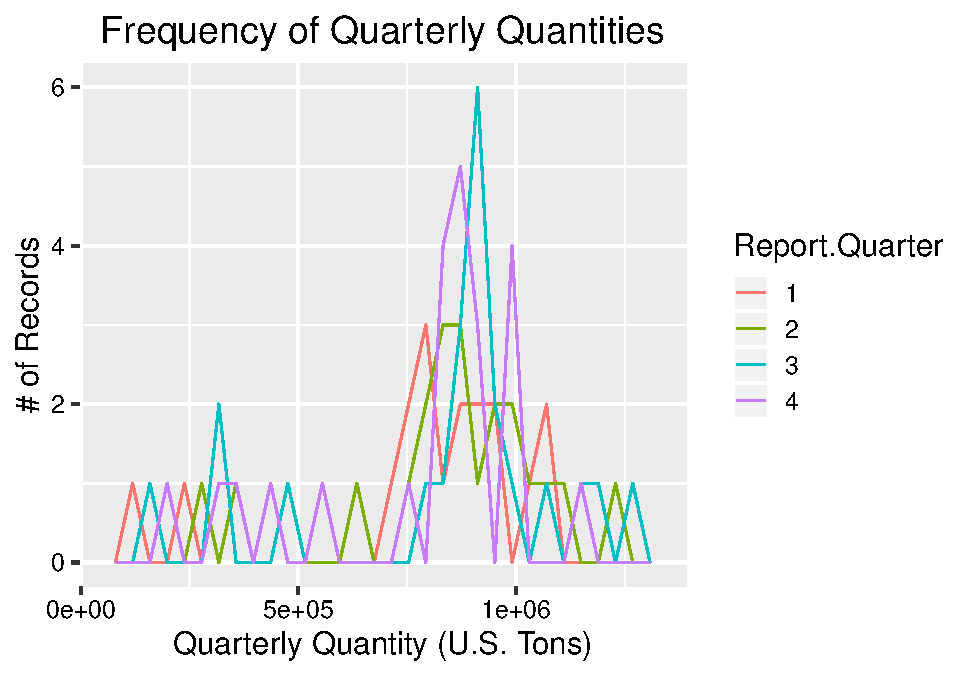
\includegraphics{SKo_Project_Template_files/figure-latex/Test1-1.pdf}

\begin{Shaded}
\begin{Highlighting}[]
\KeywordTok{qqnorm}\NormalTok{(ADC_total_only}\OperatorTok{$}\NormalTok{Total); }\KeywordTok{qqline}\NormalTok{(ADC_total_only}\OperatorTok{$}\NormalTok{Total) }\CommentTok{# does not match 1:1 ratio}
\end{Highlighting}
\end{Shaded}

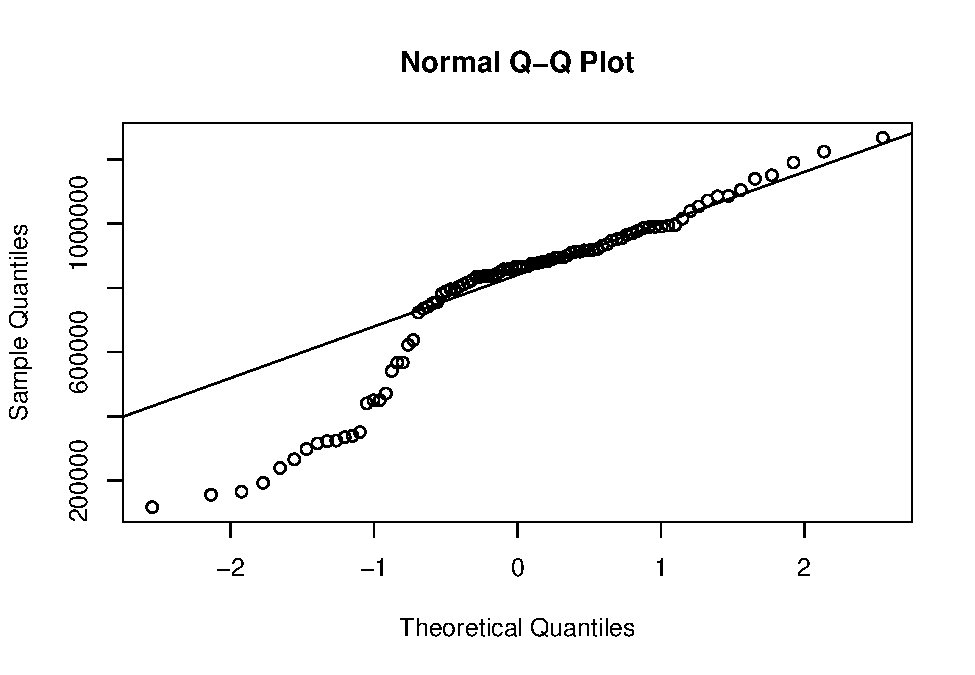
\includegraphics{SKo_Project_Template_files/figure-latex/Test1-2.pdf}

\begin{Shaded}
\begin{Highlighting}[]
\CommentTok{# Try to fix departure from normality with ln of Total. Result is not improved, so keep non-transformed data}
\NormalTok{ADC_LogTotal <-}\StringTok{ }\KeywordTok{mutate}\NormalTok{(ADC_total_only, }\DataTypeTok{LogTotal =} \KeywordTok{log}\NormalTok{(Total))}
\KeywordTok{qqnorm}\NormalTok{(ADC_LogTotal}\OperatorTok{$}\NormalTok{LogTotal); }\KeywordTok{qqline}\NormalTok{(ADC_LogTotal}\OperatorTok{$}\NormalTok{LogTotal)}
\end{Highlighting}
\end{Shaded}

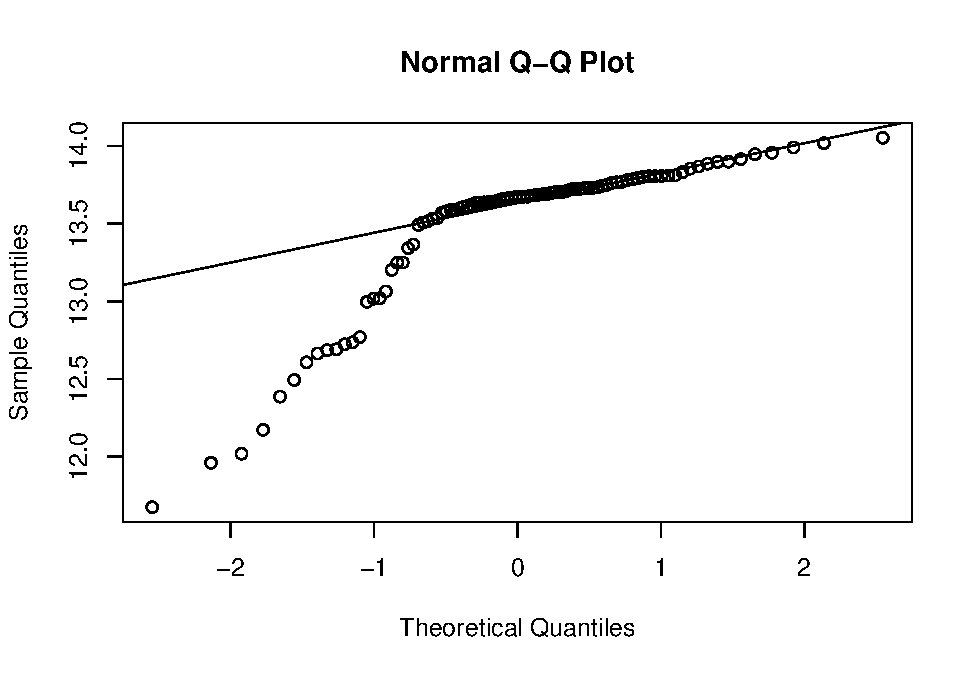
\includegraphics{SKo_Project_Template_files/figure-latex/Test1-3.pdf}

\begin{Shaded}
\begin{Highlighting}[]
\KeywordTok{bartlett.test}\NormalTok{(ADC_LogTotal}\OperatorTok{$}\NormalTok{LogTotal }\OperatorTok{~}\StringTok{ }\NormalTok{ADC_LogTotal}\OperatorTok{$}\NormalTok{Report.Quarter)}
\end{Highlighting}
\end{Shaded}

\begin{verbatim}
## 
##  Bartlett test of homogeneity of variances
## 
## data:  ADC_LogTotal$LogTotal by ADC_LogTotal$Report.Quarter
## Bartlett's K-squared = 1.1435, df = 3, p-value = 0.7666
\end{verbatim}

\begin{Shaded}
\begin{Highlighting}[]
\CommentTok{# Try to fix departure from normality with 1/Total. Result is not improved, so keep non-transformed data}
\NormalTok{ADC_InvTotal <-}\StringTok{ }\KeywordTok{mutate}\NormalTok{(ADC_total_only, }\DataTypeTok{InvTotal =} \DecValTok{1}\OperatorTok{/}\NormalTok{Total)}
\KeywordTok{qqnorm}\NormalTok{(ADC_InvTotal}\OperatorTok{$}\NormalTok{InvTotal); }\KeywordTok{qqline}\NormalTok{(ADC_InvTotal}\OperatorTok{$}\NormalTok{InvTotal)}
\end{Highlighting}
\end{Shaded}

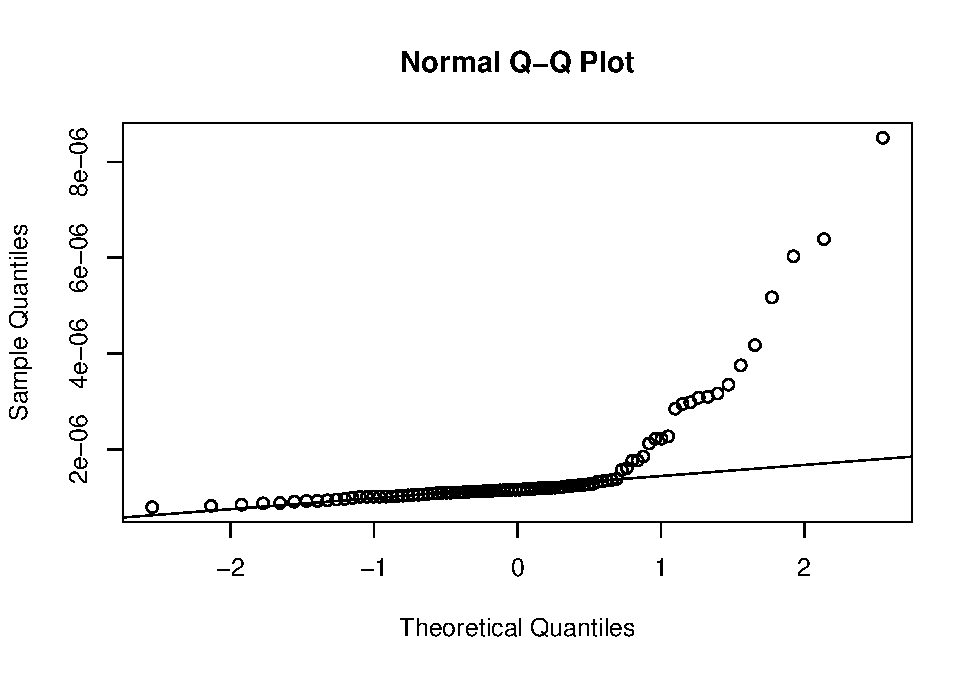
\includegraphics{SKo_Project_Template_files/figure-latex/Test1-4.pdf}

\begin{Shaded}
\begin{Highlighting}[]
\KeywordTok{bartlett.test}\NormalTok{(ADC_InvTotal}\OperatorTok{$}\NormalTok{InvTotal }\OperatorTok{~}\StringTok{ }\NormalTok{ADC_InvTotal}\OperatorTok{$}\NormalTok{Report.Quarter)}
\end{Highlighting}
\end{Shaded}

\begin{verbatim}
## 
##  Bartlett test of homogeneity of variances
## 
## data:  ADC_InvTotal$InvTotal by ADC_InvTotal$Report.Quarter
## Bartlett's K-squared = 6.519, df = 3, p-value = 0.08892
\end{verbatim}

\begin{Shaded}
\begin{Highlighting}[]
\CommentTok{# test assumption #2: equal variances among groups}

\CommentTok{# null hypothesis is that the variance is the same for the treatment groups}
\KeywordTok{bartlett.test}\NormalTok{(ADC_total_only}\OperatorTok{$}\NormalTok{Total }\OperatorTok{~}\StringTok{ }\NormalTok{ADC_total_only}\OperatorTok{$}\NormalTok{Report.Quarter) }\CommentTok{#p-value = 0.9308 # df = 3 (statistical power is very low)}
\end{Highlighting}
\end{Shaded}

\begin{verbatim}
## 
##  Bartlett test of homogeneity of variances
## 
## data:  ADC_total_only$Total by ADC_total_only$Report.Quarter
## Bartlett's K-squared = 0.44478, df = 3, p-value = 0.9308
\end{verbatim}

\begin{Shaded}
\begin{Highlighting}[]
\CommentTok{# dataset is not normal, but does fulfill requirement for same variances. proceed with non-parametric tests.}

\CommentTok{# try non-parametric w/ post hoc, bc sample size is on the smaller end for parametric}
\NormalTok{ADC_quarter_kw <-}\StringTok{ }\KeywordTok{kruskal.test}\NormalTok{(ADC_total_only}\OperatorTok{$}\NormalTok{Total }\OperatorTok{~}\StringTok{ }\NormalTok{ADC_total_only}\OperatorTok{$}\NormalTok{Report.Quarter)}
\NormalTok{ADC_quarter_kw}
\end{Highlighting}
\end{Shaded}

\begin{verbatim}
## 
##  Kruskal-Wallis rank sum test
## 
## data:  ADC_total_only$Total by ADC_total_only$Report.Quarter
## Kruskal-Wallis chi-squared = 3.4581, df = 3, p-value = 0.3262
\end{verbatim}

\begin{Shaded}
\begin{Highlighting}[]
\KeywordTok{dunnTest}\NormalTok{(ADC_total_only}\OperatorTok{$}\NormalTok{Total, ADC_total_only}\OperatorTok{$}\NormalTok{Report.Quarter)}
\end{Highlighting}
\end{Shaded}

\begin{verbatim}
##   Comparison           Z    P.unadj     P.adj
## 1      1 - 2 -1.08778370 0.27669061 1.0000000
## 2      1 - 3 -1.84978446 0.06434462 0.3860677
## 3      2 - 3 -0.76200076 0.44605955 0.8921191
## 4      1 - 4 -1.00495753 0.31491730 1.0000000
## 5      2 - 4  0.08282617 0.93398976 0.9339898
## 6      3 - 4  0.84482693 0.39820748 1.0000000
\end{verbatim}

\begin{Shaded}
\begin{Highlighting}[]
\CommentTok{# plot the results}
\NormalTok{ADC_quarter_plot <-}\StringTok{ }\KeywordTok{ggplot}\NormalTok{(ADC_total_only, }\KeywordTok{aes}\NormalTok{(}\DataTypeTok{x =}\NormalTok{ Report.Quarter, }\DataTypeTok{y =}\NormalTok{ Total)) }\OperatorTok{+}
\StringTok{  }\KeywordTok{geom_violin}\NormalTok{(}\DataTypeTok{draw_quantiles =} \FloatTok{0.5}\NormalTok{) }\OperatorTok{+}\StringTok{ }
\StringTok{  }\KeywordTok{xlab}\NormalTok{(}\StringTok{'Report Quarter'}\NormalTok{) }\OperatorTok{+}\StringTok{ }
\StringTok{  }\KeywordTok{ylab}\NormalTok{(}\StringTok{'Quantity (U.S. Tons)'}\NormalTok{) }\OperatorTok{+}\StringTok{ }
\StringTok{  }\KeywordTok{ggtitle}\NormalTok{(}\StringTok{'ADC Quantities by Quarter'}\NormalTok{)}
\KeywordTok{print}\NormalTok{(ADC_quarter_plot)}
\end{Highlighting}
\end{Shaded}

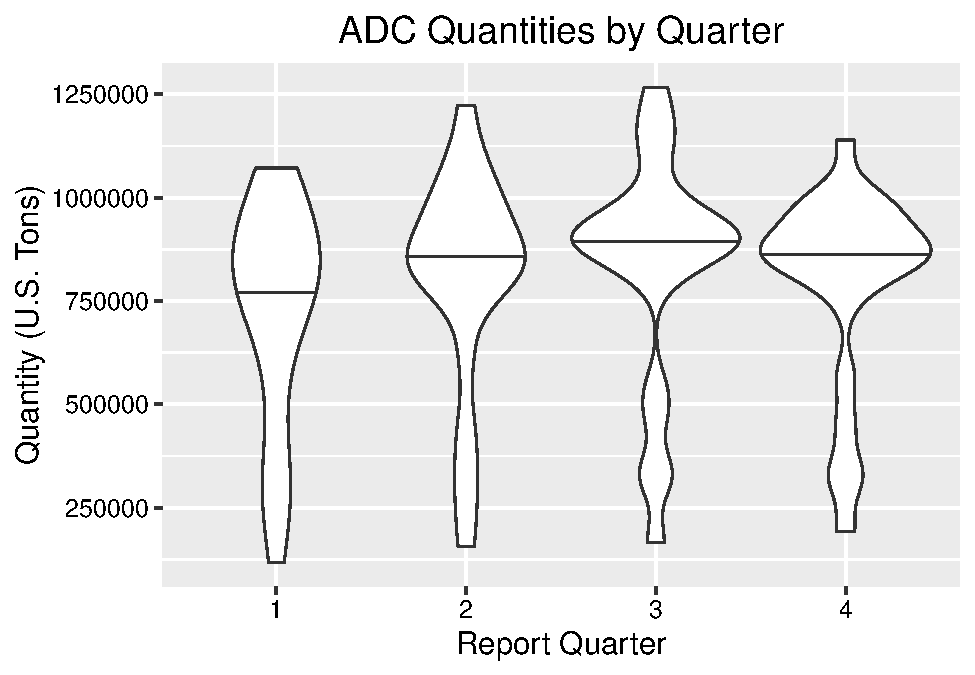
\includegraphics{SKo_Project_Template_files/figure-latex/Test1-5.pdf}

\begin{Shaded}
\begin{Highlighting}[]
\CommentTok{# save figure}
\KeywordTok{ggsave}\NormalTok{(}\StringTok{"QuarterlyADC_violinplot.jpg"}\NormalTok{, ADC_quarter_plot, }\DataTypeTok{path =} \StringTok{"../Output"}\NormalTok{, }\DataTypeTok{height =} \DecValTok{4}\NormalTok{, }\DataTypeTok{width =} \DecValTok{6}\NormalTok{, }\DataTypeTok{units =} \StringTok{"in"}\NormalTok{, }\DataTypeTok{dpi =} \DecValTok{300}\NormalTok{)}
\end{Highlighting}
\end{Shaded}

\subsection{Test 2: Statistical Modeling \& Data
Visualization}\label{test-2-statistical-modeling-data-visualization}

Can total annual ADC be represented with a linear model?

\begin{Shaded}
\begin{Highlighting}[]
\CommentTok{# assumptions for lm (independent observation, normal distribution, equal variances among groups) checked in Test 1. data is not normal, but group variances are equal. proceed with lm}

\CommentTok{# create dates corresponding to year & quarter combination}
\CommentTok{# Q1: Mar 31}
\CommentTok{# Q2: Jun 30}
\CommentTok{# Q3: Sep 30}
\CommentTok{# Q4: Dec 31}

\CommentTok{# create dataframe of month-date}
\NormalTok{quarters_to_dates <-}\StringTok{ }\KeywordTok{data.frame}\NormalTok{(}\StringTok{"Quarter"}\NormalTok{ =}\StringTok{ }\KeywordTok{as.factor}\NormalTok{(}\DecValTok{1}\OperatorTok{:}\DecValTok{4}\NormalTok{), }\StringTok{"Month.Date"}\NormalTok{ =}\StringTok{ }\KeywordTok{c}\NormalTok{(}\StringTok{'3-31'}\NormalTok{, }\StringTok{'6-30'}\NormalTok{, }\StringTok{'9-30'}\NormalTok{, }\StringTok{'12-31'}\NormalTok{))}

\CommentTok{# create new dataframe with dates}
\NormalTok{ADC_fulldate <-}\StringTok{ }\NormalTok{ADC_total_only }\OperatorTok\StringTok{ }
\StringTok{  }\KeywordTok{inner_join}\NormalTok{(quarters_to_dates, }\DataTypeTok{by =} \KeywordTok{c}\NormalTok{(}\StringTok{"Report.Quarter"}\NormalTok{ =}\StringTok{  "Quarter"}\NormalTok{)) }\OperatorTok
\StringTok{  }\KeywordTok{unite}\NormalTok{(}\StringTok{'Quarter.End.Date'}\NormalTok{, }\KeywordTok{c}\NormalTok{(Report.Year, Month.Date), }\DataTypeTok{sep =} \StringTok{"-"}\NormalTok{, }\DataTypeTok{remove =} \OtherTok{FALSE}\NormalTok{)}

\NormalTok{ADC_fulldate}\OperatorTok{$}\NormalTok{Quarter.End.Date <-}\StringTok{ }\KeywordTok{as.Date}\NormalTok{(ADC_fulldate}\OperatorTok{$}\NormalTok{Quarter.End.Date, }\StringTok{"%Y-%m-%d"}\NormalTok{)}
\KeywordTok{class}\NormalTok{(ADC_fulldate}\OperatorTok{$}\NormalTok{Quarter.End.Date)}
\end{Highlighting}
\end{Shaded}

\begin{verbatim}
## [1] "Date"
\end{verbatim}

\begin{Shaded}
\begin{Highlighting}[]
\CommentTok{# create initial plot to visualize the data}
\KeywordTok{ggplot}\NormalTok{(ADC_fulldate, }\KeywordTok{aes}\NormalTok{(}\DataTypeTok{x =}\NormalTok{ Quarter.End.Date, }\DataTypeTok{y =}\NormalTok{ Total)) }\OperatorTok{+}
\StringTok{  }\KeywordTok{geom_point}\NormalTok{() }\OperatorTok{+}\StringTok{ }
\StringTok{  }\KeywordTok{xlab}\NormalTok{(}\StringTok{""}\NormalTok{) }\OperatorTok{+}\StringTok{ }
\StringTok{  }\KeywordTok{ylab}\NormalTok{(}\StringTok{"ADC Quantity (U.S. Tons)"}\NormalTok{) }\OperatorTok{+}
\StringTok{  }\KeywordTok{ggtitle}\NormalTok{(}\StringTok{"Quarterly Quantities of ADC"}\NormalTok{)}
\end{Highlighting}
\end{Shaded}

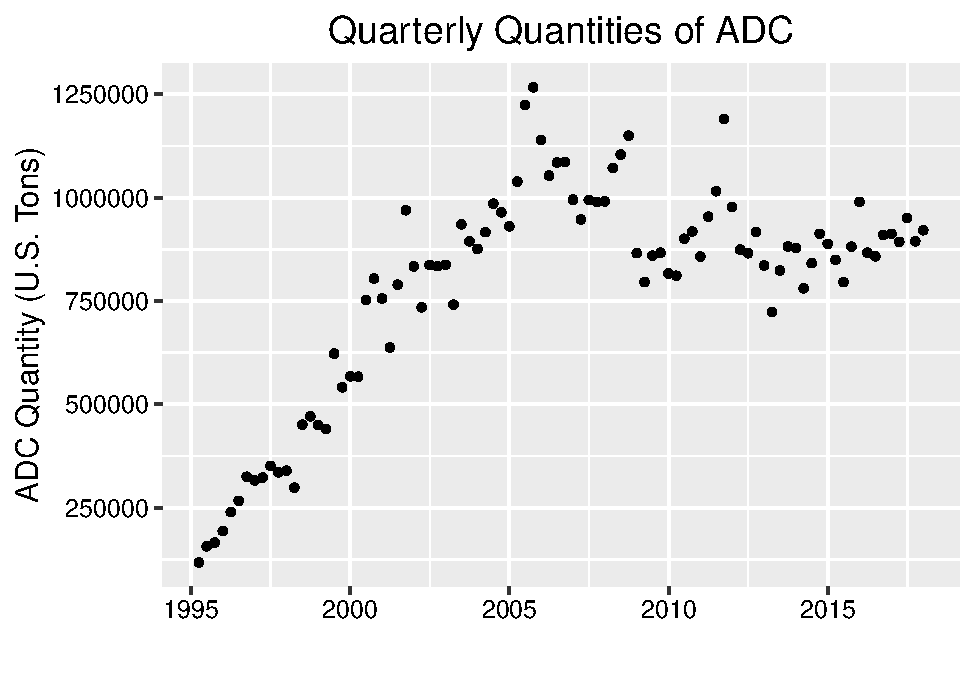
\includegraphics{SKo_Project_Template_files/figure-latex/Test2-1.pdf}

\begin{Shaded}
\begin{Highlighting}[]
\CommentTok{# create lm}
\NormalTok{ADC_date_lm <-}\StringTok{ }\KeywordTok{lm}\NormalTok{(}\DataTypeTok{data =}\NormalTok{ ADC_fulldate, Total }\OperatorTok{~}\StringTok{ }\NormalTok{Quarter.End.Date)}
\NormalTok{ADC_date_lm }\CommentTok{# Total = 73.14*Quarter.End.Date - 190264.58}
\end{Highlighting}
\end{Shaded}

\begin{verbatim}
## 
## Call:
## lm(formula = Total ~ Quarter.End.Date, data = ADC_fulldate)
## 
## Coefficients:
##      (Intercept)  Quarter.End.Date  
##       -190264.58             73.14
\end{verbatim}

\begin{Shaded}
\begin{Highlighting}[]
\KeywordTok{summary}\NormalTok{(ADC_date_lm) }\CommentTok{# Adjusted R-squared:  0.4433 (date explains 44.33% of variation in total), p-value: 2.694e-13}
\end{Highlighting}
\end{Shaded}

\begin{verbatim}
## 
## Call:
## lm(formula = Total ~ Quarter.End.Date, data = ADC_fulldate)
## 
## Residuals:
##     Min      1Q  Median      3Q     Max 
## -366483 -153515  -45160  167108  502499 
## 
## Coefficients:
##                    Estimate Std. Error t value Pr(>|t|)    
## (Intercept)      -1.903e+05  1.160e+05   -1.64    0.104    
## Quarter.End.Date  7.314e+01  8.534e+00    8.57 2.69e-13 ***
## ---
## Signif. codes:  0 '***' 0.001 '**' 0.01 '*' 0.05 '.' 0.1 ' ' 1
## 
## Residual standard error: 198500 on 90 degrees of freedom
## Multiple R-squared:  0.4494, Adjusted R-squared:  0.4433 
## F-statistic: 73.45 on 1 and 90 DF,  p-value: 2.694e-13
\end{verbatim}

\begin{Shaded}
\begin{Highlighting}[]
\CommentTok{# check normality of residuals}
\KeywordTok{par}\NormalTok{(}\DataTypeTok{mfrow=}\KeywordTok{c}\NormalTok{(}\DecValTok{2}\NormalTok{,}\DecValTok{2}\NormalTok{))}
\KeywordTok{plot}\NormalTok{(ADC_date_lm) }\CommentTok{# QQ of residuals looks relatively normal}
\end{Highlighting}
\end{Shaded}

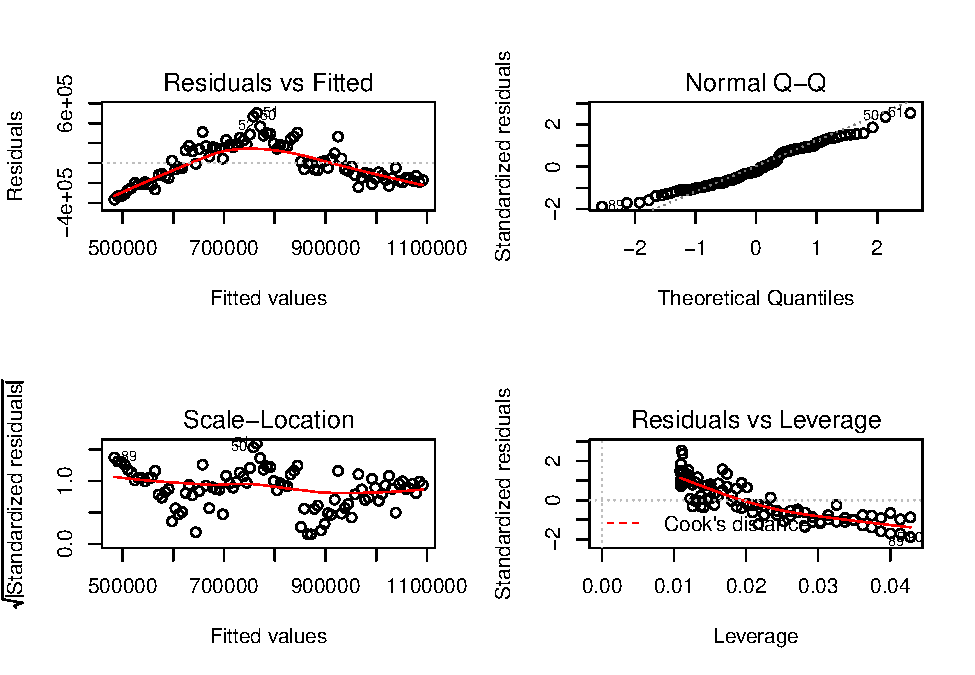
\includegraphics{SKo_Project_Template_files/figure-latex/Test2-2.pdf}

\begin{Shaded}
\begin{Highlighting}[]
\CommentTok{# plot data w/ model}
\NormalTok{ADC_fulldate_plot <-}\StringTok{ }\KeywordTok{ggplot}\NormalTok{(ADC_fulldate, }\KeywordTok{aes}\NormalTok{(}\DataTypeTok{x =}\NormalTok{ Quarter.End.Date, }\DataTypeTok{y =}\NormalTok{ Total)) }\OperatorTok{+}
\StringTok{  }\KeywordTok{geom_abline}\NormalTok{(}\DataTypeTok{intercept =} \OperatorTok{-}\FloatTok{190264.58}\NormalTok{, }\DataTypeTok{slope =} \FloatTok{73.14}\NormalTok{) }\OperatorTok{+}\StringTok{ }
\StringTok{  }\KeywordTok{geom_point}\NormalTok{() }\OperatorTok{+}\StringTok{ }
\StringTok{  }\KeywordTok{xlab}\NormalTok{(}\StringTok{''}\NormalTok{) }\OperatorTok{+}\StringTok{ }
\StringTok{  }\KeywordTok{ylab}\NormalTok{(}\StringTok{'Quarterly Quantity (U.S. Tons)'}\NormalTok{) }\OperatorTok{+}\StringTok{ }
\StringTok{  }\KeywordTok{ggtitle}\NormalTok{(}\StringTok{'Quarterly Quantities of ADC'}\NormalTok{) }
\KeywordTok{print}\NormalTok{(ADC_fulldate_plot)}
\end{Highlighting}
\end{Shaded}

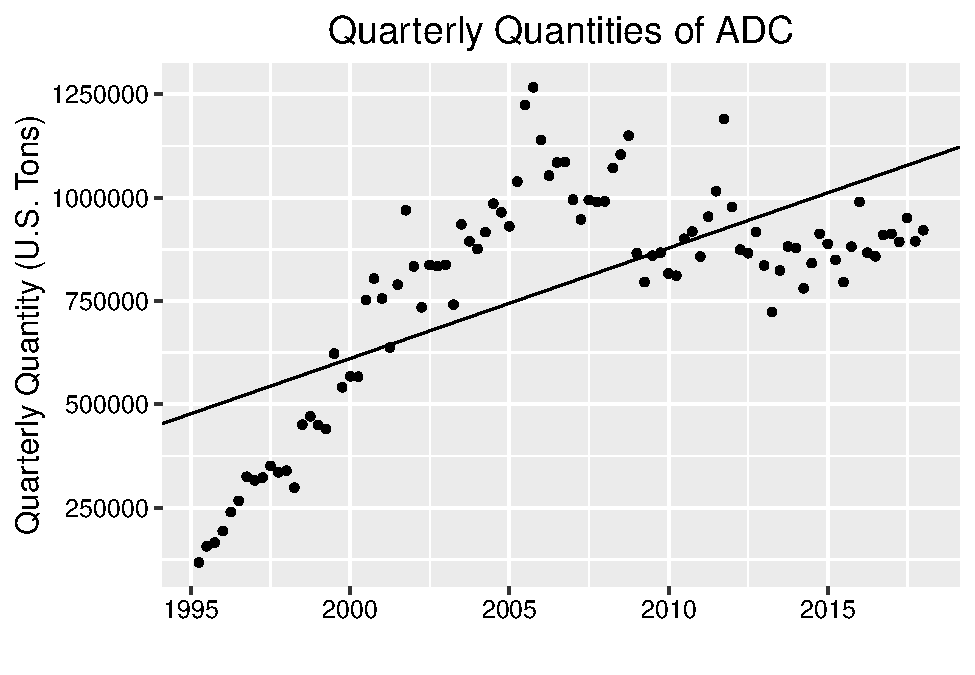
\includegraphics{SKo_Project_Template_files/figure-latex/Test2-3.pdf}

\begin{Shaded}
\begin{Highlighting}[]
\CommentTok{# visually, model does not appear to be a great fit}

\CommentTok{# save figure}
\KeywordTok{ggsave}\NormalTok{(}\StringTok{"TotalADC_plot_calculatedmodel.jpg"}\NormalTok{, ADC_fulldate_plot, }\DataTypeTok{path =} \StringTok{"../Output"}\NormalTok{, }\DataTypeTok{height =} \DecValTok{4}\NormalTok{, }\DataTypeTok{width =} \DecValTok{6}\NormalTok{, }\DataTypeTok{units =} \StringTok{"in"}\NormalTok{, }\DataTypeTok{dpi =} \DecValTok{300}\NormalTok{)}

\CommentTok{# plot with loess smoother}
\NormalTok{ADC_fulldate_plot_loess <-}\StringTok{ }\KeywordTok{ggplot}\NormalTok{(ADC_fulldate, }\KeywordTok{aes}\NormalTok{(}\DataTypeTok{x =}\NormalTok{ Quarter.End.Date, }\DataTypeTok{y =}\NormalTok{ Total)) }\OperatorTok{+}
\StringTok{  }\KeywordTok{geom_point}\NormalTok{() }\OperatorTok{+}\StringTok{ }
\StringTok{  }\KeywordTok{geom_smooth}\NormalTok{(}\DataTypeTok{method =}\NormalTok{ loess) }\OperatorTok{+}
\StringTok{  }\KeywordTok{xlab}\NormalTok{(}\StringTok{''}\NormalTok{) }\OperatorTok{+}\StringTok{ }
\StringTok{  }\KeywordTok{ylab}\NormalTok{(}\StringTok{'Quarterly Quantity (U.S. Tons)'}\NormalTok{) }\OperatorTok{+}\StringTok{ }
\StringTok{  }\KeywordTok{ggtitle}\NormalTok{(}\StringTok{'Quarterly Quantities of ADC'}\NormalTok{) }
\KeywordTok{print}\NormalTok{(ADC_fulldate_plot_loess)}
\end{Highlighting}
\end{Shaded}

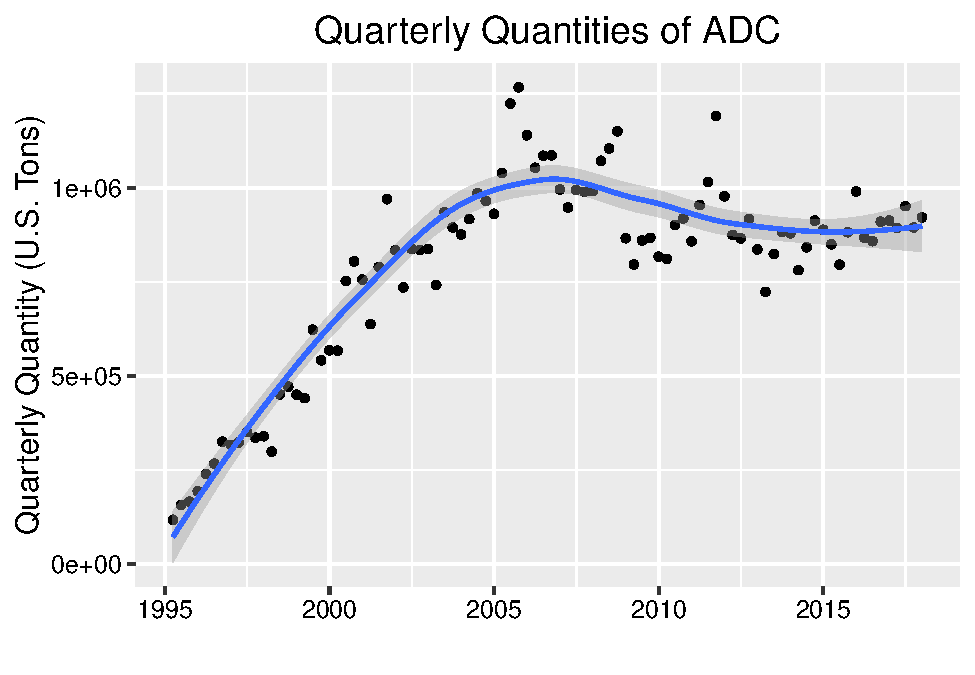
\includegraphics{SKo_Project_Template_files/figure-latex/Test2-4.pdf}

\begin{Shaded}
\begin{Highlighting}[]
\CommentTok{# visually, model appears to be a great fit}

\CommentTok{# save figure}
\KeywordTok{ggsave}\NormalTok{(}\StringTok{"TotalADC_plot_loess.jpg"}\NormalTok{, ADC_fulldate_plot_loess, }\DataTypeTok{path =} \StringTok{"../Output"}\NormalTok{, }\DataTypeTok{height =} \DecValTok{4}\NormalTok{, }\DataTypeTok{width =} \DecValTok{6}\NormalTok{, }\DataTypeTok{units =} \StringTok{"in"}\NormalTok{, }\DataTypeTok{dpi =} \DecValTok{300}\NormalTok{)}
\end{Highlighting}
\end{Shaded}

\subsection{Test 3: Statistical Modeling \& Data
Visualization}\label{test-3-statistical-modeling-data-visualization}

Is there a changepoint in the Construction \& Demolition quantities over
time?

\begin{Shaded}
\begin{Highlighting}[]
\CommentTok{# create dataframe with dates}
\NormalTok{quarters_to_dates}\OperatorTok{$}\NormalTok{Quarter <-}\StringTok{ }\KeywordTok{as.integer}\NormalTok{(quarters_to_dates}\OperatorTok{$}\NormalTok{Quarter)}

\NormalTok{CD_only <-}\StringTok{ }\NormalTok{ADC_data }\OperatorTok\StringTok{ }
\StringTok{  }\KeywordTok{select}\NormalTok{(Report.Year, Report.Quarter, Construction.and.Demolition.Waste) }\OperatorTok
\StringTok{  }\KeywordTok{inner_join}\NormalTok{(quarters_to_dates, }\DataTypeTok{by =} \KeywordTok{c}\NormalTok{(}\StringTok{"Report.Quarter"}\NormalTok{ =}\StringTok{  "Quarter"}\NormalTok{)) }\OperatorTok
\StringTok{  }\KeywordTok{unite}\NormalTok{(}\StringTok{'Quarter.End.Date'}\NormalTok{, }\KeywordTok{c}\NormalTok{(Report.Year, Month.Date), }\DataTypeTok{sep =} \StringTok{"-"}\NormalTok{) }\OperatorTok
\StringTok{  }\KeywordTok{select}\NormalTok{(}\OperatorTok{-}\NormalTok{Report.Quarter)}

\NormalTok{CD_only}\OperatorTok{$}\NormalTok{Quarter.End.Date <-}\StringTok{ }\KeywordTok{as.Date}\NormalTok{(CD_only}\OperatorTok{$}\NormalTok{Quarter.End.Date, }\StringTok{'%Y-%m-%d'}\NormalTok{) }\CommentTok{# format column as date}

\CommentTok{# arrange data from oldest to newest}
\NormalTok{CD_only <-}\StringTok{ }\NormalTok{CD_only }\OperatorTok\StringTok{ }
\StringTok{  }\KeywordTok{arrange}\NormalTok{(Quarter.End.Date)}

\CommentTok{# create initial plot to visualize the data}
\KeywordTok{ggplot}\NormalTok{(CD_only, }\KeywordTok{aes}\NormalTok{(}\DataTypeTok{x =}\NormalTok{ Quarter.End.Date, }\DataTypeTok{y =}\NormalTok{ Construction.and.Demolition.Waste)) }\OperatorTok{+}
\StringTok{  }\KeywordTok{geom_point}\NormalTok{() }\OperatorTok{+}\StringTok{ }
\StringTok{  }\KeywordTok{xlab}\NormalTok{(}\StringTok{""}\NormalTok{) }\OperatorTok{+}\StringTok{ }
\StringTok{  }\KeywordTok{ylab}\NormalTok{(}\StringTok{"C&D Quantity (U.S. Tons)"}\NormalTok{) }\OperatorTok{+}\StringTok{ }
\StringTok{  }\KeywordTok{ggtitle}\NormalTok{(}\StringTok{"Construction & Demolition Quarterly Quantities"}\NormalTok{)}
\end{Highlighting}
\end{Shaded}

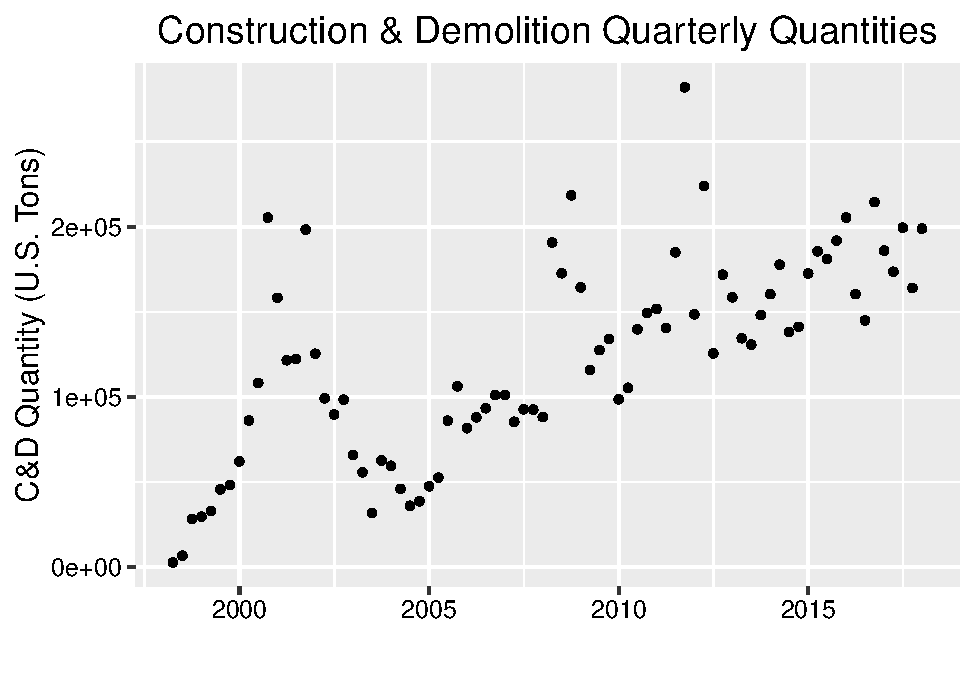
\includegraphics{SKo_Project_Template_files/figure-latex/Test3-1.pdf}

\begin{Shaded}
\begin{Highlighting}[]
\CommentTok{# check normality for C&D waste specifically}
\KeywordTok{shapiro.test}\NormalTok{(CD_only}\OperatorTok{$}\NormalTok{Construction.and.Demolition.Waste) }\CommentTok{# p-value = 0.4028, inferring that the data is normal}
\end{Highlighting}
\end{Shaded}

\begin{verbatim}
## 
##  Shapiro-Wilk normality test
## 
## data:  CD_only$Construction.and.Demolition.Waste
## W = 0.9837, p-value = 0.4028
\end{verbatim}

\begin{Shaded}
\begin{Highlighting}[]
\KeywordTok{ggplot}\NormalTok{(CD_only) }\OperatorTok{+}
\StringTok{  }\KeywordTok{geom_histogram}\NormalTok{(}\KeywordTok{aes}\NormalTok{(}\DataTypeTok{x =}\NormalTok{ Construction.and.Demolition.Waste)) }\OperatorTok{+}\StringTok{ }
\StringTok{  }\KeywordTok{xlab}\NormalTok{(}\StringTok{"Quarterly C&D (U.S. Tons)"}\NormalTok{) }\OperatorTok{+}
\StringTok{  }\KeywordTok{ylab}\NormalTok{(}\StringTok{"Count"}\NormalTok{) }\OperatorTok{+}\StringTok{ }
\StringTok{  }\KeywordTok{ggtitle}\NormalTok{(}\StringTok{"Count of Quarterly C&D Quantities"}\NormalTok{)}
\end{Highlighting}
\end{Shaded}

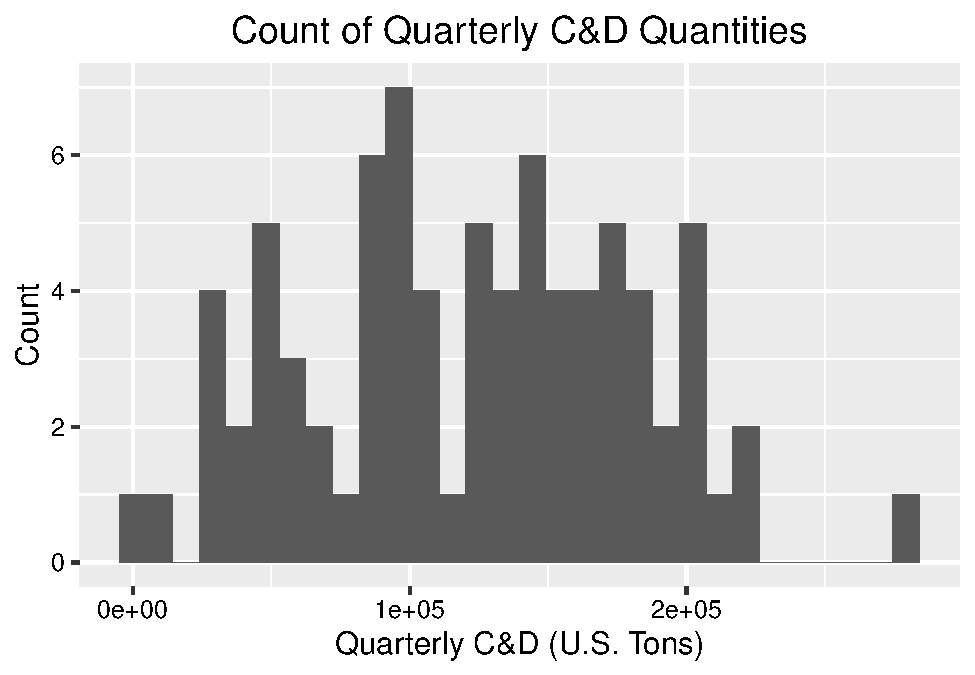
\includegraphics{SKo_Project_Template_files/figure-latex/Test3-2.pdf}

\begin{Shaded}
\begin{Highlighting}[]
\KeywordTok{qqnorm}\NormalTok{(CD_only}\OperatorTok{$}\NormalTok{Construction.and.Demolition.Waste); }\KeywordTok{qqline}\NormalTok{(CD_only}\OperatorTok{$}\NormalTok{Construction.and.Demolition.Waste) }\CommentTok{# matches 1:1 ratio pretty well}
\end{Highlighting}
\end{Shaded}

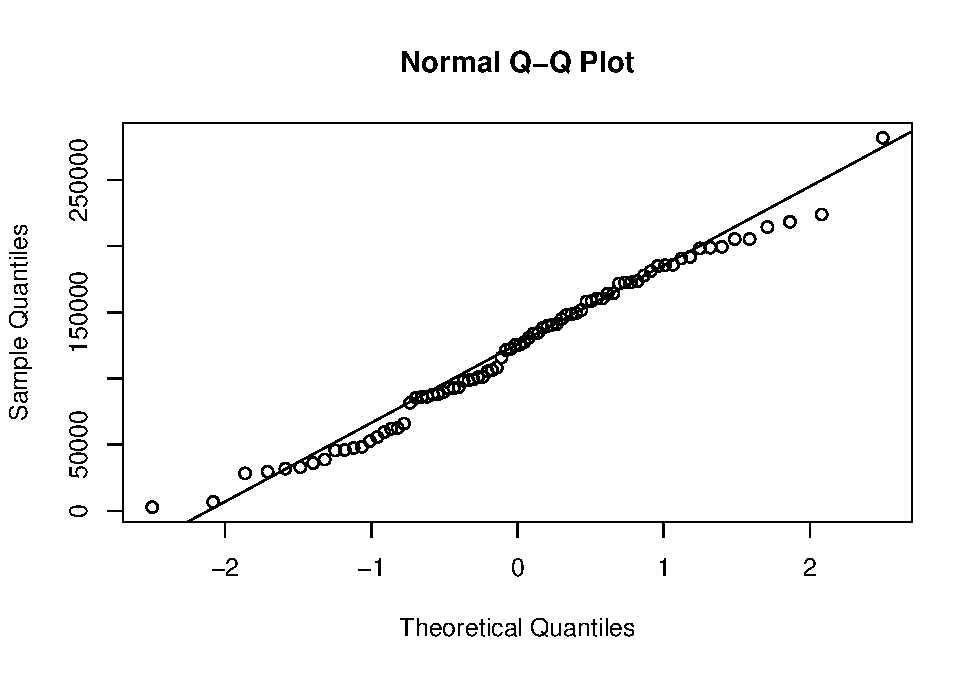
\includegraphics{SKo_Project_Template_files/figure-latex/Test3-3.pdf}

\begin{Shaded}
\begin{Highlighting}[]
\CommentTok{# use Pettitt's test (nonparametric) to determine whether there is a shift in the central tendency of the time series. }
\KeywordTok{pettitt.test}\NormalTok{(CD_only}\OperatorTok{$}\NormalTok{Construction.and.Demolition.Waste) }\CommentTok{# change point at time 40}
\end{Highlighting}
\end{Shaded}

\begin{verbatim}
## 
##  Pettitt's test for single change-point detection
## 
## data:  CD_only$Construction.and.Demolition.Waste
## U* = 1396, p-value = 3.2e-10
## alternative hypothesis: two.sided
## sample estimates:
## probable change point at time K 
##                              40
\end{verbatim}

\begin{Shaded}
\begin{Highlighting}[]
\CommentTok{# Run separate Mann-Kendall for each section}
\KeywordTok{mk.test}\NormalTok{(CD_only}\OperatorTok{$}\NormalTok{Construction.and.Demolition.Waste[}\DecValTok{1}\OperatorTok{:}\DecValTok{40}\NormalTok{])}
\end{Highlighting}
\end{Shaded}

\begin{verbatim}
## 
##  Mann-Kendall trend test
## 
## data:  CD_only$Construction.and.Demolition.Waste[1:40]
## z = 1.736, n = 40, p-value = 0.08256
## alternative hypothesis: true S is not equal to 0
## sample estimates:
##            S         varS          tau 
##  150.0000000 7366.6666667    0.1923077
\end{verbatim}

\begin{Shaded}
\begin{Highlighting}[]
\KeywordTok{mk.test}\NormalTok{(CD_only}\OperatorTok{$}\NormalTok{Construction.and.Demolition.Waste[}\DecValTok{41}\OperatorTok{:}\DecValTok{80}\NormalTok{])}
\end{Highlighting}
\end{Shaded}

\begin{verbatim}
## 
##  Mann-Kendall trend test
## 
## data:  CD_only$Construction.and.Demolition.Waste[41:80]
## z = 2.4817, n = 40, p-value = 0.01308
## alternative hypothesis: true S is not equal to 0
## sample estimates:
##           S        varS         tau 
##  214.000000 7366.666667    0.274359
\end{verbatim}

\begin{Shaded}
\begin{Highlighting}[]
\CommentTok{# Is there a second change point?}
\KeywordTok{pettitt.test}\NormalTok{(CD_only}\OperatorTok{$}\NormalTok{Construction.and.Demolition.Waste[}\DecValTok{41}\OperatorTok{:}\DecValTok{80}\NormalTok{])}
\end{Highlighting}
\end{Shaded}

\begin{verbatim}
## 
##  Pettitt's test for single change-point detection
## 
## data:  CD_only$Construction.and.Demolition.Waste[41:80]
## U* = 203, p-value = 0.04614
## alternative hypothesis: two.sided
## sample estimates:
## probable change point at time K 
##                              27
\end{verbatim}

\begin{Shaded}
\begin{Highlighting}[]
\CommentTok{# position 27, so 41+27 = change point at time 68}

\CommentTok{# Run separate Mann-Kendall for new section}
\KeywordTok{mk.test}\NormalTok{(CD_only}\OperatorTok{$}\NormalTok{Construction.and.Demolition.Waste[}\DecValTok{69}\OperatorTok{:}\DecValTok{80}\NormalTok{]) }\CommentTok{# p-value = 0.9453, not likely a 3rd change point}
\end{Highlighting}
\end{Shaded}

\begin{verbatim}
## 
##  Mann-Kendall trend test
## 
## data:  CD_only$Construction.and.Demolition.Waste[69:80]
## z = 0.068573, n = 12, p-value = 0.9453
## alternative hypothesis: true S is not equal to 0
## sample estimates:
##            S         varS          tau 
##   2.00000000 212.66666667   0.03030303
\end{verbatim}

\begin{Shaded}
\begin{Highlighting}[]
\CommentTok{# Is there a third change point?}
\KeywordTok{pettitt.test}\NormalTok{(CD_only}\OperatorTok{$}\NormalTok{Construction.and.Demolition.Waste[}\DecValTok{69}\OperatorTok{:}\DecValTok{80}\NormalTok{]) }\CommentTok{# p-value = p-value = 1.261, no 3rd change point}
\end{Highlighting}
\end{Shaded}

\begin{verbatim}
## 
##  Pettitt's test for single change-point detection
## 
## data:  CD_only$Construction.and.Demolition.Waste[69:80]
## U* = 12, p-value = 1.261
## alternative hypothesis: two.sided
## sample estimates:
## probable change point at time K 
##                               6
\end{verbatim}

\begin{Shaded}
\begin{Highlighting}[]
\CommentTok{# years corresponding to changepoints}
\NormalTok{changepoint1 <-}\StringTok{ }\NormalTok{CD_only}\OperatorTok{$}\NormalTok{Quarter.End.Date[}\DecValTok{40}\NormalTok{] }\CommentTok{# between Q4 2007 & Q1 2008 = ~ 2008-02-14}
\NormalTok{changepoint2 <-}\StringTok{ }\NormalTok{CD_only}\OperatorTok{$}\NormalTok{Quarter.End.Date[}\DecValTok{68}\NormalTok{] }\CommentTok{# between Q4 2014 & Q1 2015 = ~ 2015-02-14}

\CommentTok{# Add vertical lines to the original graph to represent change points}
\NormalTok{CD_plot_changepoints <-}\StringTok{ }\KeywordTok{ggplot}\NormalTok{(CD_only, }\KeywordTok{aes}\NormalTok{(}\DataTypeTok{x=}\NormalTok{Quarter.End.Date, }\DataTypeTok{y=}\NormalTok{Construction.and.Demolition.Waste)) }\OperatorTok{+}
\StringTok{  }\KeywordTok{geom_point}\NormalTok{() }\OperatorTok{+}
\StringTok{  }\KeywordTok{geom_vline}\NormalTok{(}\KeywordTok{aes}\NormalTok{(}\DataTypeTok{xintercept=}\KeywordTok{as.Date}\NormalTok{(}\StringTok{'2008-02-14'}\NormalTok{)), }\DataTypeTok{linetype=}\DecValTok{2}\NormalTok{, }\DataTypeTok{colour=}\StringTok{"purple"}\NormalTok{, }\DataTypeTok{size=}\DecValTok{1}\NormalTok{) }\OperatorTok{+}
\StringTok{  }\KeywordTok{geom_vline}\NormalTok{(}\KeywordTok{aes}\NormalTok{(}\DataTypeTok{xintercept=}\KeywordTok{as.Date}\NormalTok{(}\StringTok{'2015-02-14'}\NormalTok{)), }\DataTypeTok{linetype=}\DecValTok{4}\NormalTok{, }\DataTypeTok{colour=}\StringTok{"blue"}\NormalTok{, }\DataTypeTok{size=}\DecValTok{1}\NormalTok{) }\OperatorTok{+}\StringTok{ }
\StringTok{  }\KeywordTok{geom_text}\NormalTok{(}\DataTypeTok{x=}\KeywordTok{as.Date}\NormalTok{(}\StringTok{'2010-1-1'}\NormalTok{), }\DataTypeTok{y=}\DecValTok{260000}\NormalTok{, }\DataTypeTok{label=}\NormalTok{stringr}\OperatorTok{::}\KeywordTok{str_wrap}\NormalTok{(}\StringTok{'changepoint1: Q4,2007-Q1,2008'}\NormalTok{, }\DecValTok{15}\NormalTok{), }\DataTypeTok{colour=}\StringTok{"purple"}\NormalTok{, }\DataTypeTok{size=}\DecValTok{5}\NormalTok{) }\OperatorTok{+}
\StringTok{  }\KeywordTok{geom_text}\NormalTok{(}\DataTypeTok{x=}\KeywordTok{as.Date}\NormalTok{(}\StringTok{'2017-1-1'}\NormalTok{), }\DataTypeTok{y=}\DecValTok{260000}\NormalTok{, }\DataTypeTok{label=}\NormalTok{stringr}\OperatorTok{::}\KeywordTok{str_wrap}\NormalTok{(}\StringTok{'changepoint2: Q4,2014-Q1,2015'}\NormalTok{, }\DecValTok{15}\NormalTok{), }\DataTypeTok{colour=}\StringTok{"blue"}\NormalTok{, }\DataTypeTok{size=}\DecValTok{5}\NormalTok{) }\OperatorTok{+}
\StringTok{  }\KeywordTok{xlab}\NormalTok{(}\StringTok{''}\NormalTok{) }\OperatorTok{+}
\StringTok{  }\KeywordTok{ylab}\NormalTok{(}\StringTok{'Quarterly C&D Cover (U.S. Tons)'}\NormalTok{) }\OperatorTok{+}\StringTok{ }
\StringTok{  }\KeywordTok{scale_y_continuous}\NormalTok{(}\DataTypeTok{labels =}\NormalTok{ scales}\OperatorTok{::}\NormalTok{comma) }\OperatorTok{+}\StringTok{ }
\StringTok{  }\KeywordTok{ggtitle}\NormalTok{(}\StringTok{'Construction & Demolition Landfill Cover in CA'}\NormalTok{)}
\KeywordTok{print}\NormalTok{(CD_plot_changepoints)  }
\end{Highlighting}
\end{Shaded}

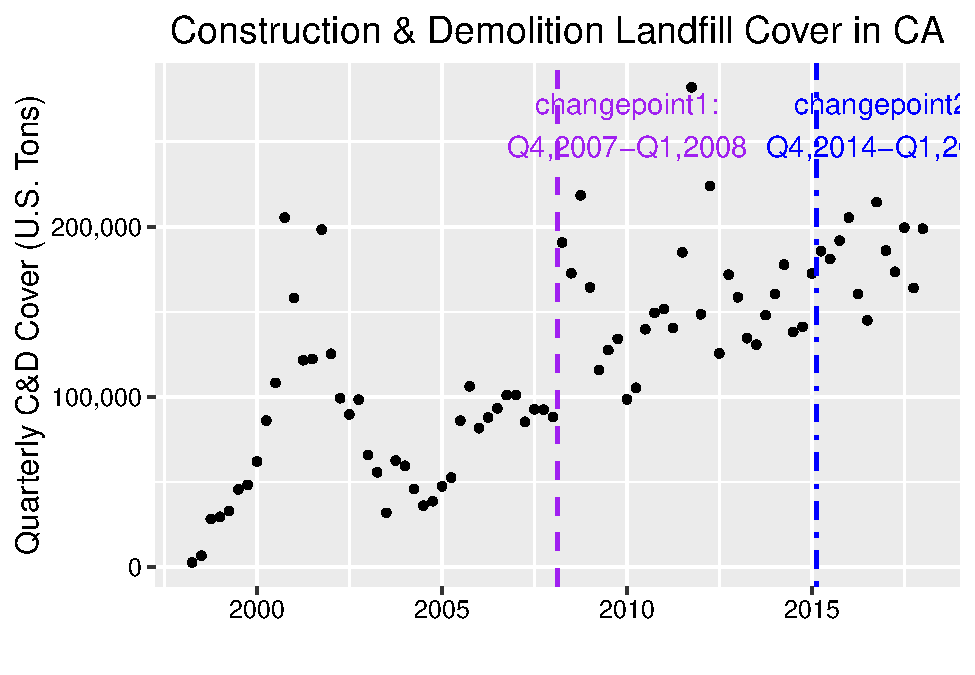
\includegraphics{SKo_Project_Template_files/figure-latex/Test3-4.pdf}

\begin{Shaded}
\begin{Highlighting}[]
\CommentTok{# save figure}
\KeywordTok{ggsave}\NormalTok{(}\StringTok{"CD_plot_changepoints.jpg"}\NormalTok{, CD_plot_changepoints, }\DataTypeTok{path =} \StringTok{"../Output"}\NormalTok{, }\DataTypeTok{height =} \DecValTok{4}\NormalTok{, }\DataTypeTok{width =} \DecValTok{11}\NormalTok{, }\DataTypeTok{units =} \StringTok{"in"}\NormalTok{, }\DataTypeTok{dpi =} \DecValTok{300}\NormalTok{)}
\end{Highlighting}
\end{Shaded}

\newpage

\section{Summary and Conclusions}\label{summary-and-conclusions}


\end{document}
